\documentclass{article}
\usepackage{polski, amsmath, pgfplots, siunitx, multirow, float, caption, graphicx}
\usepackage[hidelinks]{hyperref}
% Marginesy
\usepackage[a4paper, margin=3cm]{geometry}
% Wykresy i inne wichajstry
\pgfplotsset{width=0.8 \textwidth, max space between ticks=50pt, compat=1.18}
\pgfkeys{/pgf/number format/.cd,1000 sep={\,}, dec sep={,}}
\captionsetup[table] {labelfont={bf}, labelformat={default}, labelsep=period, name={Tab.}}
\captionsetup[figure] {labelfont={bf}, labelformat={default}, labelsep=period, name={Rys.}}

\begin{document}

\begin{center}
  \begin{huge}
    \textbf{Raport ze wstępnego etapu prac}
  \end{huge}
\end{center}

\section{Zdobycie kluczowego elementu projektu - lamp nixie}
Udało się zakupić lampy nixie w ilości 6 sztuk. Są to lampy typu Z570N, produkcji niemieckiej.
Był problem z dostępnością lamp, jednak udało się je zakupić używane w dobrym stanie w rozsądnej cenie.

\begin{figure}[H]
    \centering
    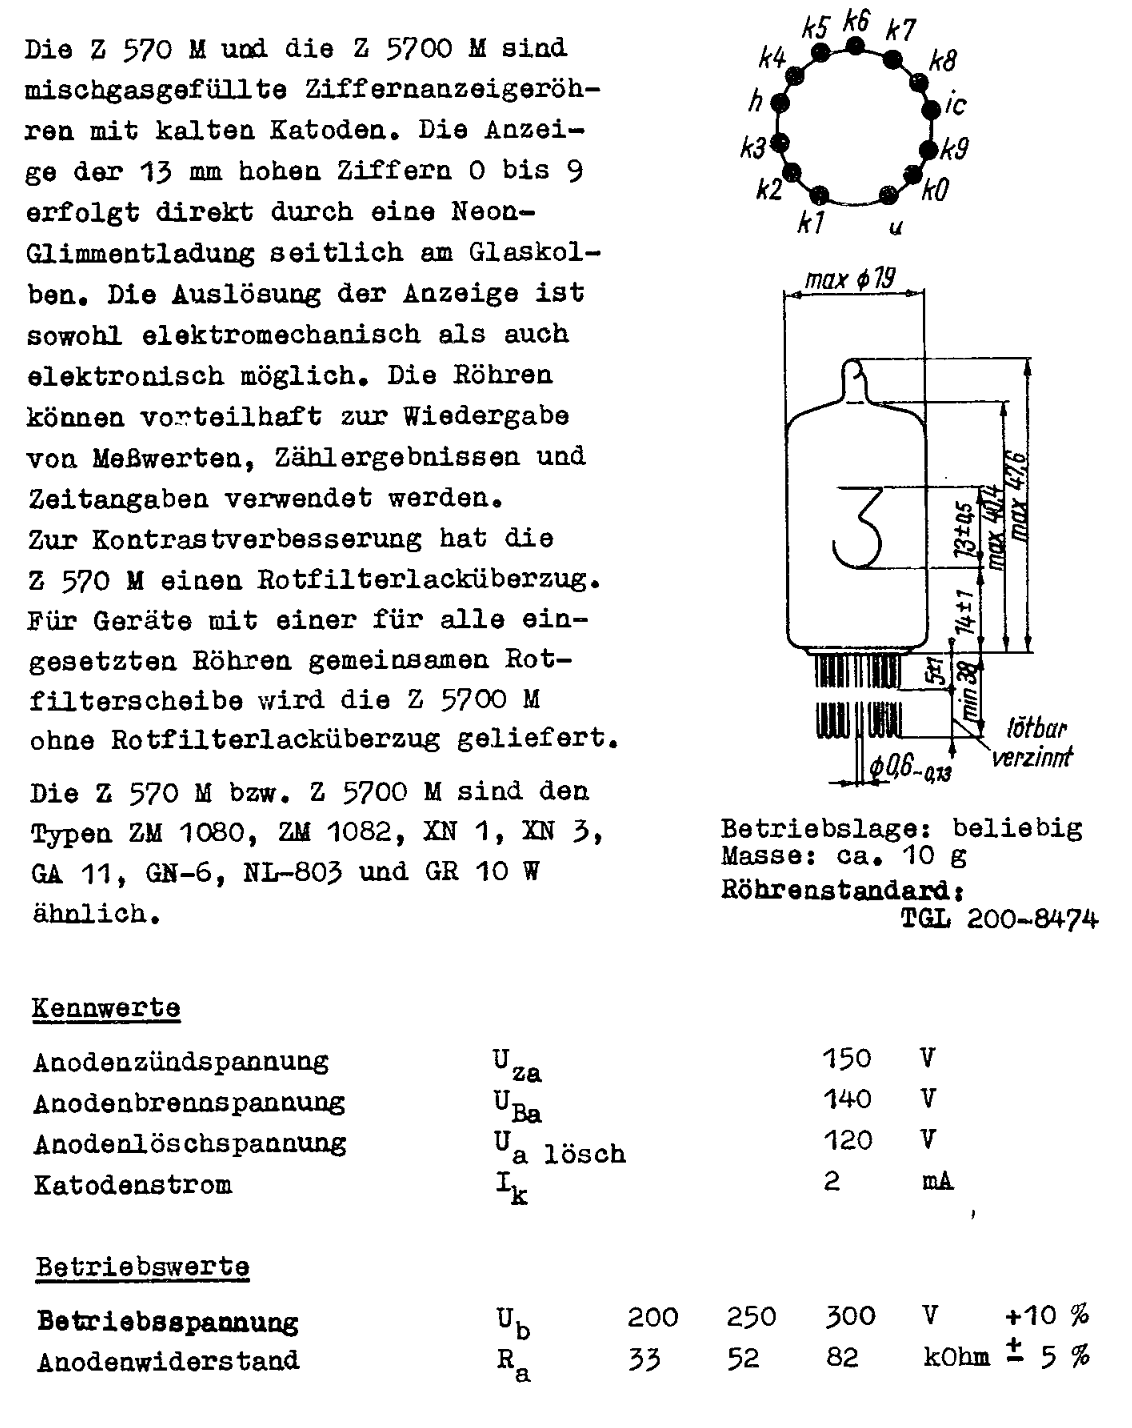
\includegraphics[width=0.6\textwidth]{doc-lamp.png}
    \caption{Fragment dokumentacji lampy nixie Z570M}
\end{figure}

\section{Opracowanie kluczowych założeń projektu}


Zegar ma być zasilany przez USB-C co wymusza zaprojektowanie konwertera zasilania z 5V na 170V co jest zadaniem trudniejszym niż z 12V na 170V\\\\
Konwerter ma mieć możliwość programowej regulacji jasności wyświetlaczy, co zostanie uzyskane poprzez regulowany dzielnik napięcia w obwodzie sprzężenia zwrotnego sterownika konwertera\\\\
By zrealizować funkcje budzika, zegar ma bedzie wyposażony w mały buzzer który będzie generował dźwięk alarmu, będzie również możliwość wykorzystania zewnętrznego głośnika bluetooth\\\\
By nie zaburzać estetyki zegara, przycisk wyłączania alarmu bedzie odzielnym modułem komyunikującym się z zegarem po jakimś prostym protokole który będzie zużywał jak najmniej energii, ponieważ przycisk będzie zasilany z baterii\\\\
Zegar ma być wyposażony w moduł WiFi, który będzie umożliwiał sterowanie zegarem z poziomu Home Assistanta, wykorzystane będą prawodopodobnie dwa mikrokontrolery, 
jeden do obsługi wyświetlaczy i przycisków, drugi n którym będzie zainstalowany ESPhome, który będzie komunikował się z Home Assistantem, a mikrokontrolery będą się komunikowac za pomocą UARTu \\\\

\section{Wstępny model 3D zegara}

\begin{figure}[H]
    \centering
    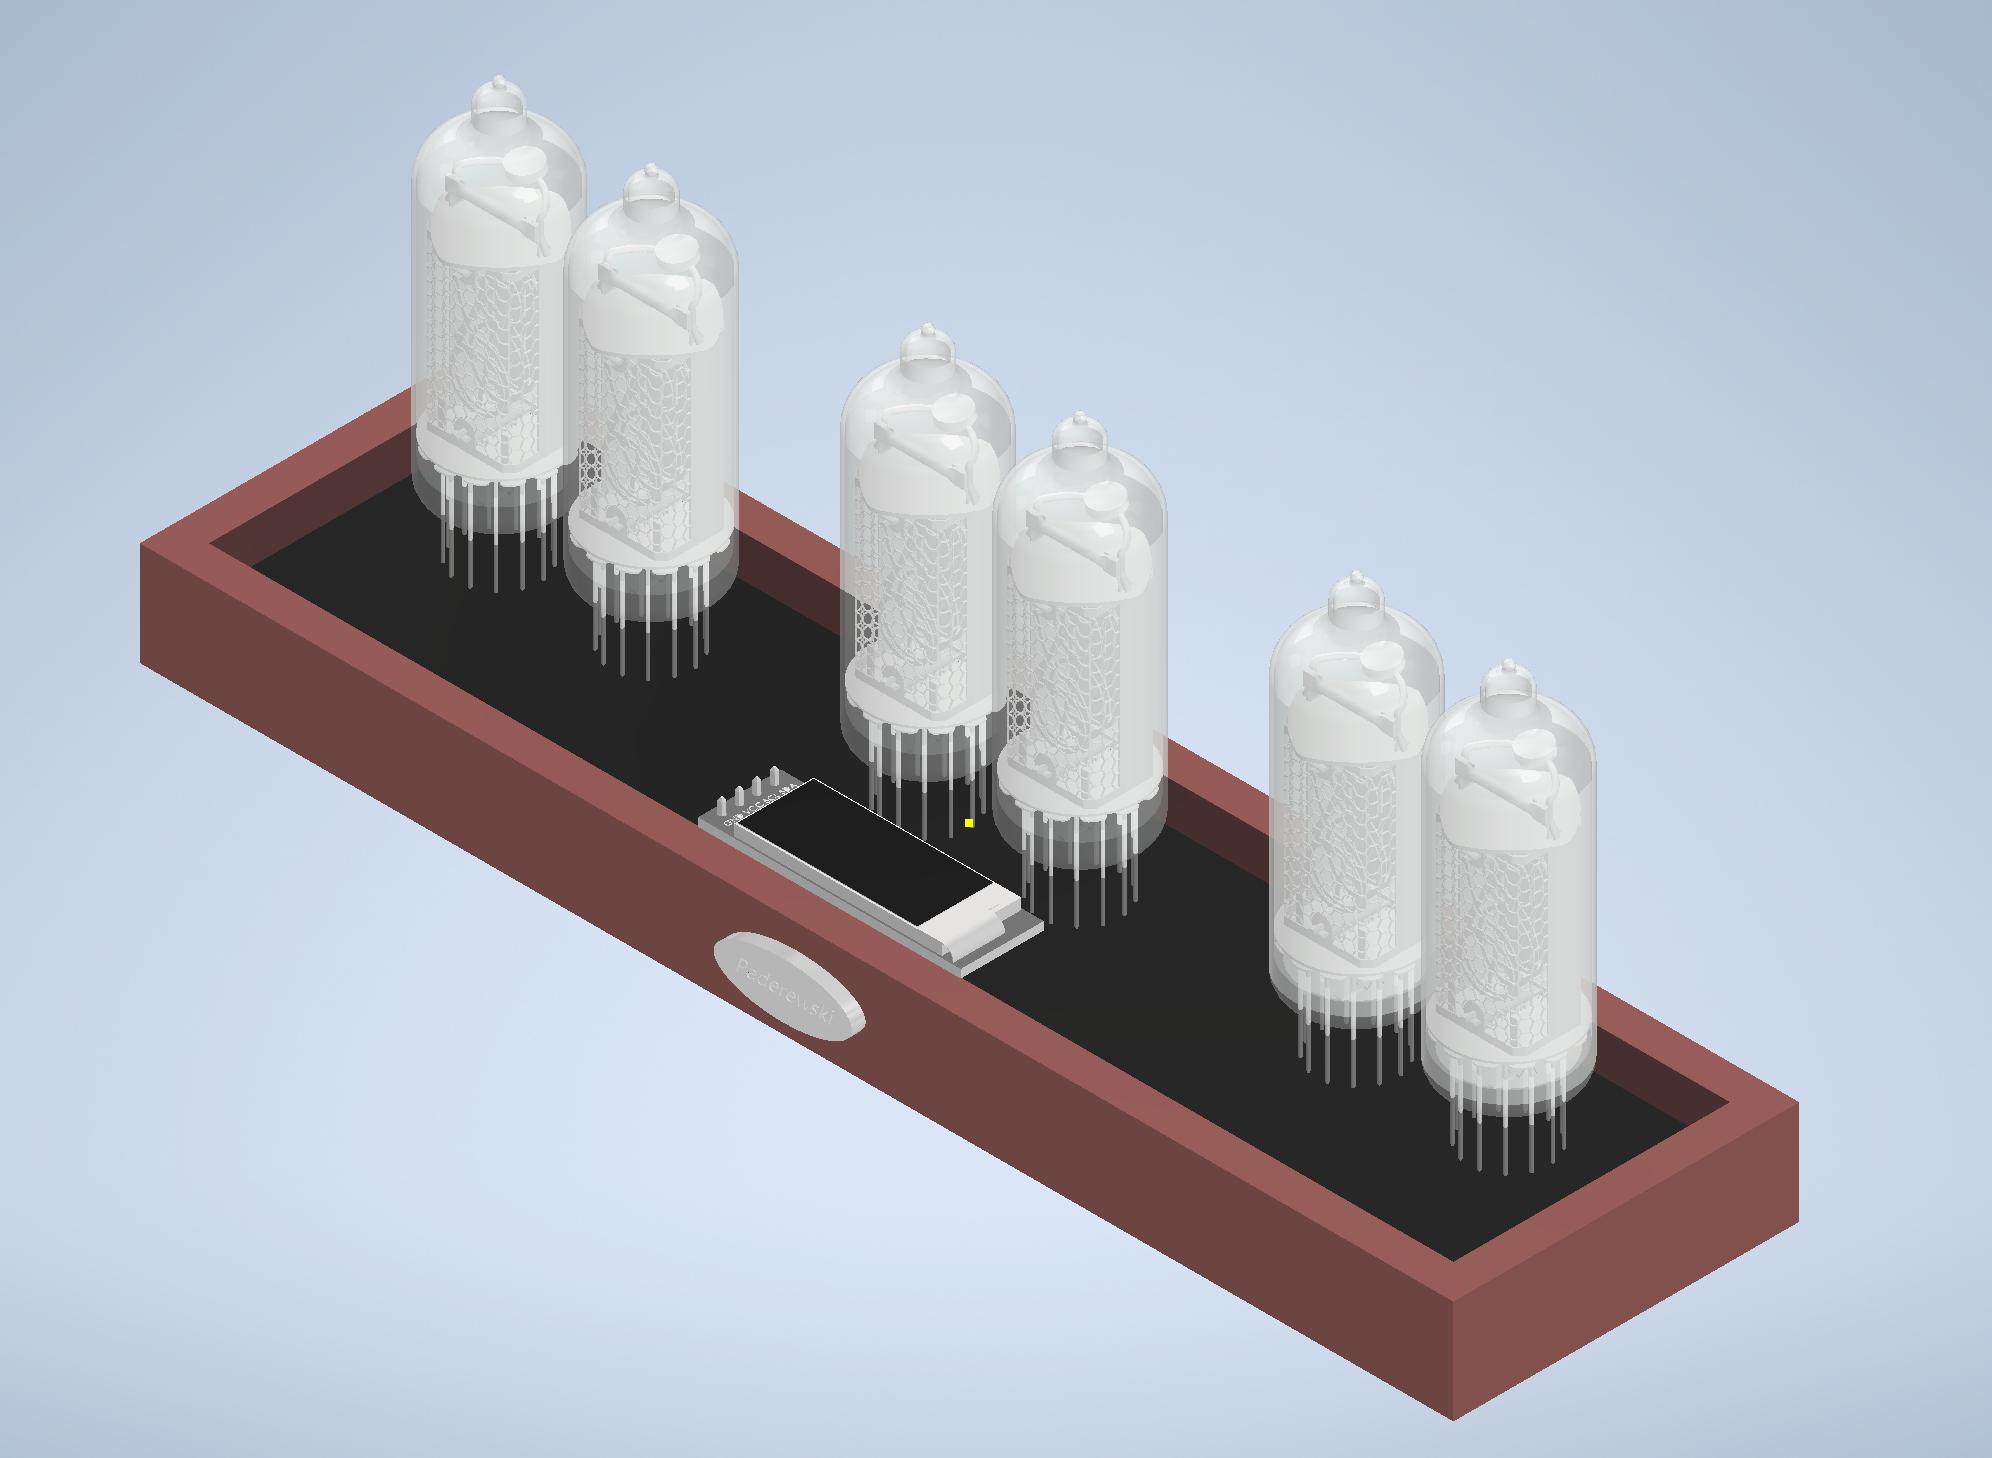
\includegraphics[width=0.6\textwidth]{model1.png}
    \caption{Wstępny model 3D zegara rzut z góry}
\end{figure}

\begin{figure}[H]
    \centering
    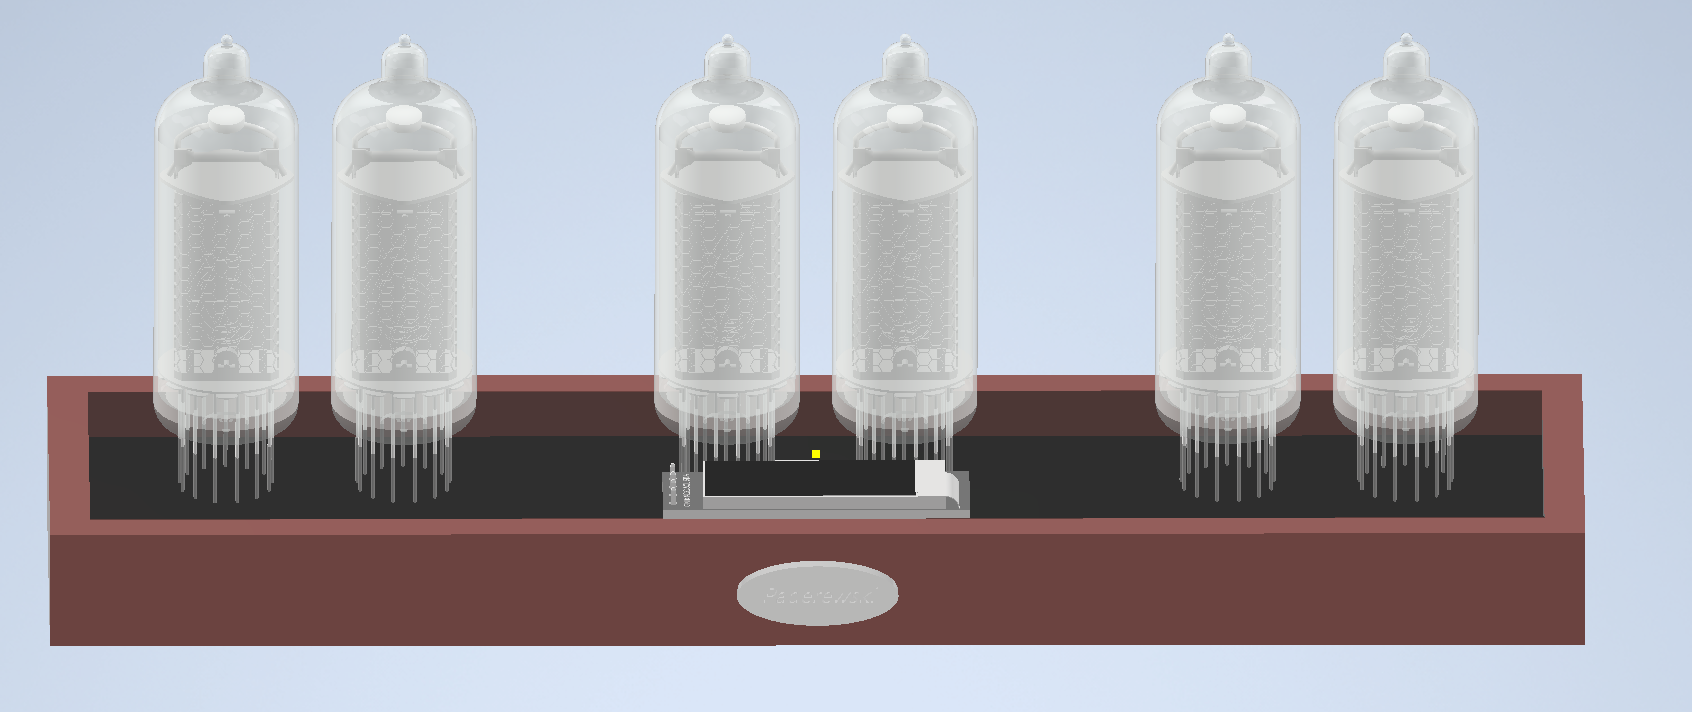
\includegraphics[width=0.6\textwidth]{model2.png}
    \caption{Wstępny model 3D zegara rzut z przodu}
\end{figure}

Model jest tylko wstępnym zarysem, aby zwizualizować jakie materiały będą użyte i jak to bedzie wyglądać.

Materiały:

\begin{itemize}
    \item Obudowa: drewno dębowe
    \item Pokrywa: szkło hartowane lub plexi (przyciemniane) ma być widoczna płytka drukowana
    \item Podstawa od spodu ma posiadać nóżki antypoślizgowe o odpowiedniej wysokości, by były widoczne ledy które będą od spodu podświetlać zegar
\end{itemize}

\section{Początek projektowania konwertera}




\end{document}
